\chapter{Trajektorien}\label{cha:trj}

\section{Einleitung}

\section{Implementierung der Trajektorienberechnung}

Die Implementierung der Trajektorienberechnung basiert auf den Erkenntnissen der Vorgängerarbeit Fauvé \cite{fauve} und erfolgt in \Matlab\ mit Hilfe des CasADi-Frameworks. Es wird einerseits auf eine Erhöhung der Modularisierung im Vergleich zur Vorgängerarbeit geachtet, andererseits werden weitere Funktionalitäten ergänzt, um die Trajektorienberechnung für die Anwendungen im Rahmen dieser Arbeit zu optimieren.

Die Berechnung der Trajektorien wird durch fünf Matlab-Funktionen modularisiert:
\begin{itemize}
	\item \textit{searchTrajectories}
	\item \textit{calculateTrajectory}
	\item \textit{getODE}
	\item \textit{getInitDev}
	\item \textit{determineAPinit}
\end{itemize}

Vom Anwender aufgerufen wird lediglich\textit{searchTrajectories}. Die weiteren vier Funktionen werden auch für andere Anwendungen dieser Arbeit eingesetzt, wodurch das Kopieren von Code vermieden wird. Änderungen, die mehrere Funktionen und Skripte betreffen, können daher effizient an einer Stelle im Programmcode durchgeführt werden. Die Argumente der Funktionen werden so gewählt, dass die in dieser Arbeit zu untersuchenden Parameter leicht durch den Funktionsaufruf in einer Schleife variiert werden können. Weitere Parameter die im Rahmen dieser Arbeit innerhalb der Funktionen konstant festgelegt sind, können zu einem späteren Zeitpunkt jedoch leicht zu den Funktionsargumenten ergänzt werden.

Im Folgenden werden die beiden wichtigsten Funktionen \textit{searchTrajectories} und \textit{calculateTrajectory} genauer beschrieben, wobei auch auf die Verwendung von \textit{getODE}, \textit{getInitDev} und \textit{determineAPinit} eingegangen wird.

\subsection{searchTrajectories}\label{subsec:searchtrj}

Durch die Funktion \textit{searchTrajectories} wird vom Anwender eine Trajektoriensuche in Auftrag gegeben. Als Beispiel für die Anwendung kann der folgende Programmcode eines \Matlab-Skriptes betrachtet werden:

\lstinputlisting[style=Matlab_colored]{Bilder/Trajektorien/Demo_searchTrajectories.m}

Zunächst wird ein Suchprogramm ausgewählt. Es kann zwischen drei Programmen ausgewählt werden:

\begin{enumerate}
	\item Suche nach der im Rahmen dieser Arbeit definierten Vergleichstrajektorie
	\item Suche nach der Aufschwungtrajektorie mit der Variationsstrategie
	\item Suche nach allen 12 Trajektorien mit der Variationsstrategie
\end{enumerate}

Dem Ansatz der Programmauswahl liegen die Erkenntnisse von Fauvé \cite{fauve} bezüglich einer Variationsstrategie zu Grunde. Da auf Grund der nichtlinearen MPC nur lokal optimiert wird, kann je nach Anfangswert ein anderes Optimum erreicht werden. Eine Variation des Anfangswertes ermöglicht somit eine effektive Suche nach Trajektorien für einen bestimmten Arbeitspunktwechsel. Im Code-Beispiel ist Suchprogramm 2 ausgewählt, der gesuchte Arbeitspunktwechsel ist allgemein der Aufschwung von AP1 nach AP4. Hierbei können innerhalb einer Periode vier mögliche Winkelanfangsauslenkungen gegenüber AP4 variiert werden, die als Startwert AP1 definieren:
\[
	\begin{bmatrix}
		0 \\ 0 \\ \pi \\ 0 \\ \pi \\ 0
	\end{bmatrix}, \quad
	\begin{bmatrix}
		0 \\ 0 \\ -\pi \\ 0 \\ \pi \\ 0
	\end{bmatrix}, \quad
	\begin{bmatrix}
		0 \\ 0 \\ \pi \\ 0 \\ -\pi \\ 0
	\end{bmatrix}, \quad
	\begin{bmatrix}
		0 \\ 0 \\ -\pi \\ 0 \\ -\pi \\ 0
	\end{bmatrix} .
\]
Eine weitere Variation durch Ausnutzung der $2\pi$-Periodizität bringt gemäß Fauvé \cite{fauve} hingegen keine Vorteile, sondern verlängert die Berechnungszeit bei gleichzeitig sinkender Wahrscheinlichkeit, dass der Algorithmus zu einer gültigen Lösung konvergiert. Die möglichen Anfangsauslenkungen werden über die Funktion \textit{getInitDev} aufgerufen.
Neben den Anfangsauslenkungen der Pendel hat auch die Schlittenposition Einfluss auf die Lösungsfindung. Daher wird diese mit den folgenden auf Fauvé \cite{fauve} basierenden Auslenkungen symmetrisch zur Bahnmitte variiert (siehe Tabelle \ref{tab:varpos}).
\begin{table}[h]
	\centering
		\begin{tabular}{r|l}
			$x_{0\mrm{,init}}$ & $x_{0\mrm{,end}}$ \\
			\midrule
			$-0,5$ & $0,5$	\\	
			$-0,3$ & $0,3$	\\	
			$-0,1$ & $0,1$	\\	
			   $0$ &   $0$	\\
			
		\end{tabular}
	\caption{Variation der Schlittenposition}
	\label{tab:varpos}
\end{table}

Als letzte Komponente der Variationsstrategie wird noch die Positionsbeschränkung variiert. Obwohl der Versuchsstand eine Positionsbeschränkung von $\pm0,8m$ vorgibt, ist es sinnvoll, auch diese zu variieren, da der Algorithmus sich sensitiv gegenüber den Nebenbedingungen verhält. Durch Verschärfung oder Lockerung der Positionsbeschränkung verändert sich die Optimierungslandschaft und damit die Chance eine Trajektorie zu finden. Bei Lockerungen der Beschränkung muss später immer geprüft werden, ob bei den gefundenen Trajektorie die Positionsbeschränkungen eingehalten werden. Es werden folgende von Fauve \cite{fauve} entnommene Variationen implementiert.
	\[
	-\underline{g}_{x_0} = \overline{g}_{x_0} \in \{ 0,6; \ 0,8; \ 1; \ 1,2; \ 1,4 \}  \ .
\]
Insgesamt werden bei Suchprogramm 2 somit $4 \cdot 4 \cdot 5 = 80$ Trajektorienberechnungen durchlaufen. Bei Suchprogramm 3 werden die beschriebenen Variationen auf alle zwölf Trajektorien ausgeweitet, indem der Endwert durch alle vier Arbeitspunkte iteriert und die Variation der Winkelanfangsauslenkungen um die vier zusätzlich entstehenden Kombinationen durch die Arbeitspunkte 2 und 3 erweitert wird. Insgesamt werden $8 \cdot 4 \cdot 5 \cdot 4 = 640$ Trajektorienberechnungen durchgeführt.
Im Rahmen dieser Arbeit wird eine Vergleichstrajektorie für die in Kapitel \ref{sec:trjparamtest} behandelten Parameteruntersuchungen verwendet. Diese wird mit Suchprogramm 1 berechnet.

Nachdem das Suchprogramm für die Trajektorienberechnung ausgewählt ist, werden Prädiktionshorizont, Schrittweite und Integrationsverfahren für die NMPC konfiguriert. Als Integratoren stehen das Eulerverfahren "`Euler"' und das Runge-Kutta-Verfahren "RK4"' zur Verfügung. Außerdem wird einer der in Kapitel \ref{subsec:spdparams} besprochenen Parametersätze übergeben sowie eine maximale Stellkraft definiert. Diese stellt eine weitere Variationsmöglichkeit dar, die von Fauve \cite{fauve} nicht untersucht worden ist. Daher wird sie zur manuellen Variation in den Argumenten der \textit{searchTrajectories} zur Verfügung gestellt.
Als Letztes wird noch bestimmt, ob für die Trajektorienberechnung die Coulombreibung im Schlitten bzw. in den Gelenken berücksichtigt werden soll. 

Die berechneten Trajektorien werden automatisch gespeichert. Es wird eine Namenskonvention zur Identifizierbarkeit der gespeicherten Ergebnisse eingeführt, die an folgendem Trajektoriennamen beispielhaft gezeigt wird:
	\[
	\textit{Traj14\_dev0\_-3.14\_-3.14\_x0max0.8\_Fmax410}
\]
Am Anfang steht die verallgemeinerte Trajektorienbezeichnung mit $\mrm{AP_{init}}$ und $\mrm{AP_{end}}$, wobei $\mrm{AP_{init}}$ erst noch aus den Anfangsauslenkungen abgeleitet werden muss. Dies geschieht mit Hilfe der Funktion \textit{determineAPinit}. Es folgen der Variationswert der Schlittenposition, die Winkelanfangsauslenkung von $\varphi_1$ und $\varphi_2$, die Positionsbeschränkung und die maximale Stellkraft. 
Wenn nicht anders angegeben, werden die Ergebnisse im Ordner \textit{searchResults} in einer definierten Ordnerstruktur gespeichert, deren Benennung sich nach der Konfiguration der NMPC richtet. Im obigen Beispiel werden die Ergebnisse in folgendem Unterordner gespeichert, wobei $Fc$ anzeigt, dass die Schlitten-Coulomb-Reibung in der Berechnung berücksichtigt wurde: 
	\[
	\textit{Results\_app09\_Fc\_T0.005N500\_RK4} \ .
\]

Optional kann der Funktion \textit{searchTrajectories} auch ein Pfad für den Speicherordner übergeben werden. Außerdem können zusätzliche Erweiterungen für den Trajektoriennamen übergeben werden, um später bei der Variation von Modellparametern die Variationswerte im Dateinamen zu berücksichtigen. 
Als weitere Option kann noch bestimmt werden, ob alle berechneten Trajektorien oder nur die mit gültiger Lösung gespeichert werden sollen. 


\subsection{calculateTrajectory}\label{subsec:calctrj}

Die Funktion \textit{calculateTrajectory} wird innerhalb von \textit{searchTrajectories} zur eigentlichen Berechnung einer bestimmten Trajektorie aufgerufen. Sie implementiert die NMPC mit Hilfe des CasADi-Frameworks auf Grundlage der Erkenntnisse der Vorgängerarbeit. Für detaillierte Hintergrundinformationen wird daher auf die Ausarbeitung von Fauvé \cite{fauve} verwiesen. Als Argument erwartet die Funktion eine Struktur mit verschiedenen Konfigurationsparametern, die im Quelltext ausführlich kommentiert sind.


Zunächst muss ein Optimalsteuerungsproblem (OCP) mit Zielfunktion und Nebenbedingungen definiert werden. Als Zielfunktion wird 
	\[
	\mrm{min} \ J = \sum_{i=1}^N ((x_i-x_\mrm{end})^T Q (x_i-x_\mrm{end}) + (u_i-u_\mrm{end})^T R (u_i-u_\mrm{end})) + 
	\sum_{i=2}^N (u_i-u_{i-1})^T S (u_i-u_{i-1})
\]
implementiert. Sie besteht aus dem bekannten \textsc{Lagrange}schen Güteintegral der LQ-Regelung und einem Bestrafungsterm für Änderungen in der Stellgröße, durch den hochfrequente Stellgrößenverläufe reduziert werden. Die Wahl der Gewichtungsmatrizen $Q$, $R$ und $S$ basiert auf den Erkenntnissen von Fauvé \cite{fauve}. Tests bestätigen diese Wahl, wobei $S$ etwas nach unten korrigiert wird. Die Matrizen werden anschließend nicht mehr variiert. Sie sind der Funktion \textit{calculateTrajectory} als Konfigurationsparameter zwar zu übergeben, werden in \textit{searchTrajectories} jedoch für die weiteren Anwendungen im Rahmen der Arbeit hartkodiert.
\[ 
	\mat{Q} = 
	\begin{bmatrix}
		500 & 0 & 0 & 0 & 0 & 0 \\
		0 & 0,01 & 0 & 0 & 0 & 0 \\
		0 & 0 & 100 & 0 & 0 & 0 \\
		0 & 0 & 0 & 0,1 & 0 & 0 \\
		0 & 0 & 0 & 0 & 100 & 0 \\
		0 & 0 & 0 & 0 & 0 & 0,1 \\
	\end{bmatrix} \ , \quad
	R = 5 \cdot 10^{-7} \ , \quad
	S = 1,5 \cdot 10^{-8} \\	
\]


Neben der Zielfunktion sind darüber hinaus folgende Nebenbedingungen zu implementieren:
\begin{itemize}
	\item Kontinuitätsbedingungen 
	\item Anfangsbedingung
	\item Endwertbedingung
	\item Positionsbegrenzung des Schlittens
	\item Stellkraftbegrenzung.
\end{itemize}

Dabei ist zu beachten, dass die Endwertbedingung, anders als die restlichen Nebenbedingungen, nicht als harte Grenze formuliert, sondern implizit durch die Zielfunktion angenähert wird. 

Um eine möglichst hohe Vergleichbarkeit mit der Vorgängerarbeit Fauvé \cite{fauve} zu erzielen, wird für die Systemgleichungen das Kraftmodell gewählt. Die nichtlinearen Gleichungen werden mit Hilfe der Funktion \textit{getODE} in CasADi-Symbolik zur Verfügung gestellt.

Die Stellstrombegrenzung in Abhängigkeit der Winkelgeschwindigkeit des Motors wird in Kapitel \ref{subsec:dcMotor} hergeleitet. Diese muss für die Implementierung noch in eine Stellkraftbegrenzung in Abhängigkeit der Schlittengeschwindigkeit umgerechnet werden.
Mit 
	\[
	\omega = \frac{1}{r_{32}\ K_G} \ \dot{x}_0 
\]
und 
	\[
	I = \frac{r_{32}\ K_G}{K_I} \ \cdot F
\]
kann Gleichung \eqref{eq:Ivar} in die Form
	\[
	F_{\mrm{max}} = \frac{K_I}{r_{32}\ K_G} \cdot \frac{U_{a\mrm{,max}}}{R_a} - (\frac{K_I}{r_{32}\ K_G})^2 \cdot \frac{\dot{x}_0}{R_a}
\]

gebracht werden. Gleiches gilt für \eqref{eq:Iconst}. Die Fallunterscheidung nach Vorzeichen der Bewegungsrichtung wird wie in Kapitel \ref{subsec:dcMotor} berücksichtigt. 

In CasADi sind zwei Arten von Beschränkungen zu unterscheiden: Einerseits Pfadbeschränkungen in Form von Gleichungen und Ungleichungen (z.B. Systemgleichungen), andererseits Ober- und Untergrenzen für die Wertebereiche der Optimierungsvariablen (z.B. $u_{\mrm{min}}<u<u_{\mrm{max}}$). Die konstante Stellbegrenzung durch den Spannungs-Strom-Wandler wird durch eine Begrenzung des Wertebereichs der Eingangsgröße $F$ realisiert. Die variable Stellbegrenzung durch die Gegeninduktion wird hingegen als Pfadbeschränkung in Form von Ungleichungen implementiert:
\[
	 0 \leq \frac{K_I}{r_{32}\ K_G} \cdot \frac{U_{a\mrm{,max}}}{R_a} - (\frac{K_I}{r_{32}\ K_G})^2 \cdot \frac{\dot{x}_0}{R_a} - F \ .
\]

Das zu lösende OCP wird durch Diskretisierung in ein endlich-dimensionales nichtlineares Programm (engl.: \textit{Nonlinear Programming})(NLP) überführt, was auch als direkter Ansatz bzw. "`first discretize, then optimize"' bezeichnet wird. Dies geschieht durch Einteilung des OCP in $N$ Intervalle der Schrittweite $T$, wobei $N$ als Zeit- oder Prädiktionshorizont bezeichnet wird. Als numerische Lösungsmethode wird das in Fauvé \cite{fauve} empfohlene \textit{Direct-Multiple-Shooting}-Verfahren implementiert. Neben dem Eingangsgrößenverlauf zählt bei diesem Verfahren auch der Zustandsgrößenverlauf zu den Optimierungsvariablen. Anders als beim \textit{Single Shooting} werden statt für den gesamten Prädiktionshorizont für jedes Intervall die Systemgleichungen gelöst. Dadurch wird das Randwertproblem zunächst in $N$ Anfangswertprobleme aufgelöst, die durch die Systemgleichungen und einen jeweils zu optimierenden Startwert definiert sind. Um sicherzustellen, dass die abschnittsweise gelösten Systemgleichungen einen stetigen Verlauf ergeben, werden $N$-Kontinuitätsbedingungen implementiert. Der Lösungsverlauf eines Intervalls soll zum nächsten Zeitschritt dem Startwert des nächsten Intervalls entsprechen.

Zur Lösung der Systemgleichungen werden das Euler-Verfahren und das Runge-Kutta-Verfahren 4. Ordnung implementiert. Als Lösungsverfahren für das NLP wird nach dem Beispiel von Fauvé \cite{fauve} das von CasADi bereitgestellte IPOPT-Verfahren (Innere-Punkte-Verfahren, engl.: \textit{Interior Point Optimization}) eingesetzt.

Vor Beginn der Optimierung müssen alle Optimierungsvariablen mit Startwerten initialisiert werden. Auf Grund des Multiple-Shooting-Ansatzes sind Startwerte über den gesamten Prädiktionshorizont sowohl für die Eingangsgröße als auch für den Zustandsvektor zu schätzen. Für den diskretisierten Eingang $u$ werden die Startwerte mit dem Nullvektor $u_0 = [0 \ 0 \ \ldots \ 0 ]^Tm\in \mathbb{R}^{1 \times N}$ initialisiert. Für die Zustände $\ves{x}$ wird ein S-förmiger Verlauf von $x_{\mrm{init}}$ nach $x_{\mrm{end}}$ geschätzt, da hiermit bei Fauvé \cite{fauve} gute Ergebnisse erzielt wurden. Der Verlauf wird durch Interpolation mit Hilfe der Funktion \textit{chip()} über 4  Stützstellen gewonnen. Der zu Grunde liegende Erwartung ist, dass das System erst langsam anfährt, dann stark beschleunigt und sich am Ende in der Nähe des Zielwerts nur noch langsam ändert.

Da die Funktion \textit{calculateTrajectory} eigens für die Trajektorienberechnung vorgesehen ist, wird, anders als bei Fauve \cite{fauve}, auf eine Iterationsschleife für die Anwendung als Regler verzichtet.

\section{Implementierung der Trajektorienfolgeregelung}

Zur Überprüfung der Stabilisierbarkeit der berechneten Trajektorien wird eine Trajektorienfolgeregelung als zeitvarianter Zustandsregler nach \cite{matPrakt2} realisiert. 

Dazu wird das nicht-lineare System wie in Kapitel \ref{subsec:lin} zunächst linearisiert. Die Linearisierung um die Trajektorie führt im Gegensatz zum zeitinvarianten Arbeitspunkt auf ein linear-zeitvariantes System (LZV).
	\[
	\Delta \ves{\dot{x}} = \mat{A}(t) \Delta \ves{x}(t) + \ves{b}(t) \Delta F(t)
\]

mit 
\begin{align*}
	\ves{x}(t) = \ves{x}_{\mrm{Traj}}(t) + \Delta \ves{x}(t) \\
	 F(t) = F_{\mrm{Traj}}(t) + \Delta F(t) \ .
\end{align*}

Hierfür lässt sich der linear-zeitinvariante (LZI) LQ-Reglerentwurf aus Kapitel \ref{subsec:zsr} übertragen, indem das zeitvariante Gütemaß 
	\[
	J = \int_{0}^{\infty} \Delta \ves{x}^T(t) \mat{Q} \Delta \ves{x}(t) + R \cdot \Delta F^2(t) \, dt
\]

durch Lösen der zeitvarianten \textsc{Riccati}-Differentialgleichungen
	\[
	\mat{\dot{P}}(t) = \mat{P}(t) R^{-1} b^2(t) \mat{P}(t) - \mat{P}(t) \mat{A}(t) - \mat{A}^T(t) \mat{P}(t) - \mat{Q}
\]

minimiert wird. Die Gleichungen werden als Endwertproblem rückwärts in der Zeit gelöst, wobei das System der Endlage $t=t_{\mrm{end}} = N \cdot T$ als Randwert vorgegeben wird. 

Damit lässt sich die Reglerverstärkung 
	\[
	\mat{K}(t) = R^{-1} b(t) \mat{P}(t)
\]

für das lineare, zeitvariante Regelgesetz
	\[
	\Delta F(t) = -\mat{K}(t) \ves{x}(t)
\]

berechnen.

Für die Implementierung der Linearisierung und die Berechnung der Reglerverstärkung werden die vom \emph{rtm} zur Verfügung gestellten "`common"'-Funktionen \textit{linSys} und \textit{getTrajFBController\_LQR} verwendet. Um die Regelung zu initialisieren wird das \Matlab-Skript \textit{InitTrajReg} erstellt. Die Initialisierung beinhaltet das Laden eines Modellparametersatzes und der zu simulierenden Trajektorie, die Berechnung des trajektorienspezifischen Zustandsreglers sowie die Bereitstellung der Reglerdaten für die Simulation. 

Das Simulationsmodell ist in Abbildung \ref{fig:TFR_Simulink} dargestellt.

\begin{figure}[h]
	\centering
		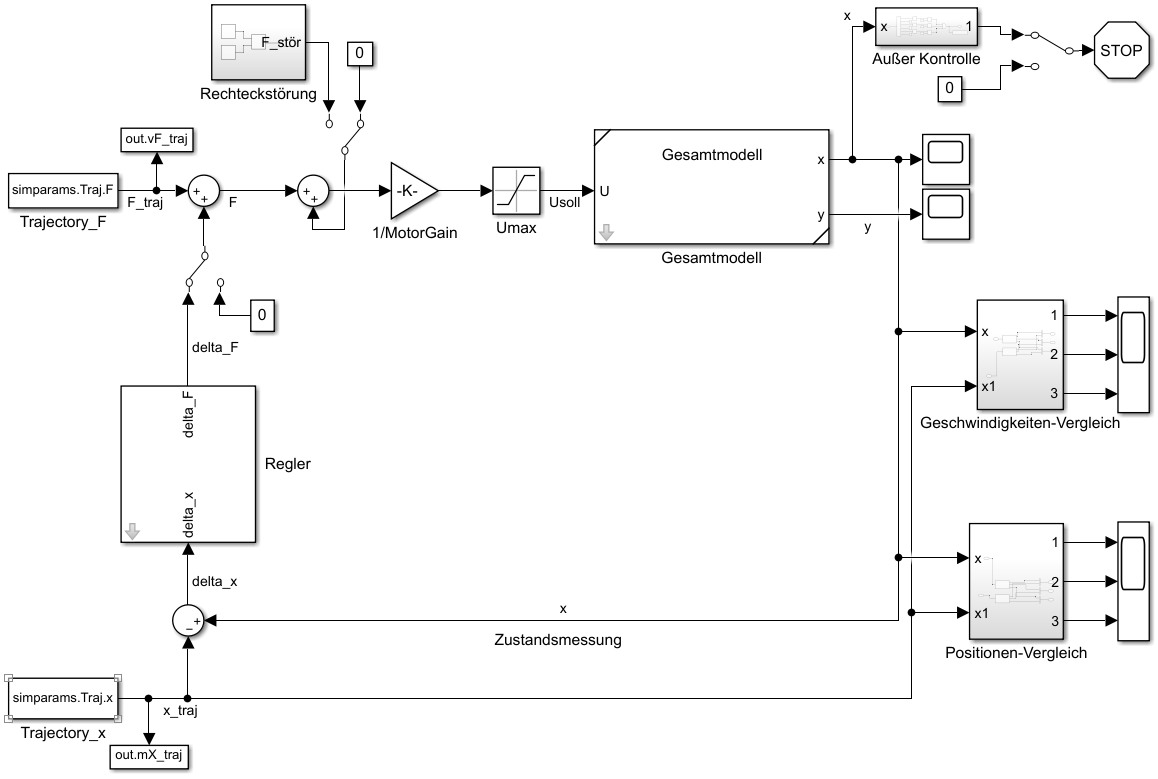
\includegraphics[width=0.98\textwidth]{Bilder/Trajektorien/TFR_Simulink.PNG}
	\caption{Trajektorienfolgeregelung in Simulink}
	\label{fig:TFR_Simulink}
\end{figure}

Die Trajektorien werden der Simulation als \textit{timeseries} mit Hilfe von \textit{From Workspace} Blöcken zugeführt. Für die anschließende Auswertung in \Matlab\ hingegen können benötigte Signale über To Workspace an \Matlab\ gereicht werden. Um instabile Simulationen zu erkennen und vorzeitig abzubrechen, wird das Subsystem \textit{Außer Kontrolle} implementiert. Optional kann die Regelung zu Vergleichszwecken abgeschaltet werden. Ebenso kann kurzzeitig eine Rechteckstörung aufgeschaltet werden. Die genannten Optionen lassen sich über \textit{Manual Switches} ein- und ausschalten, wobei deren Zustand aus \Matlab\ heraus über die Funktion \textit{set\_param} angesteuert werden kann.

\section{Stabilisierbarkeit in der Simulation}

\section{Untersuchung des Einflusses der Modellparameter}\label{sec:trjparamtest}

